\documentclass[]{article}
\usepackage{amsmath}
\usepackage{graphicx}
\usepackage{float}
%opening
\title{NCTU Machine Learning Hw1}
\author{Liang Yu Pan 0486016}

\begin{document}
	
	\maketitle
	
	
	\section{Bayesian Linear Regression}
	\paragraph{Overview}
	For Bayesian, the data is certain. So, the \textbf{w} can be viewed as uncertain distribution, so we need to integral \textbf{w}. Therefore, the problem can be transformed to be $ p(t) = \int_{\infty}^{\infty}p(t | \textbf{w}) p(\textbf{w})$. Then \textbf{w} is calculated by \textbf{x}, \textbf{t}(= $p(\textbf{w}|\textbf{x, t})$), using \textbf{maximum posterior}.  The $p(t|\textbf{w})$ is calculated by \textbf{maximum likelihood function}(= $p(t|x, \textbf{w}, \beta)$).
	\paragraph{Useful formula}
	If $p(x), p(y), p(x|y), p(y|x), $ are gaussian distribution.
	\begin{align}
	p(x) &= N(x|\mu, \Lambda^{-1})\\
	p(y|x) &= N(y|Ax+b, L^{-1})\\
	p(y) &= N(y|A\mu+b, L^{-1}+A\Lambda^{-1}A^{T})\\
	p(x|y) &= N(x|\Sigma{A^{T}L(y-b) + \Lambda\mu}, \Sigma), \Sigma = (\Lambda^{-1} + A^{T}LA^{T})^{-1}
	\end{align}
	And now we see x as \textbf{w} and y as t.
	\paragraph{Calculate $ p(w) $}
	Because $p(t|w)$ is a likelihood function of gaussian distribution given by the problem, we can assume its prior as gaussian distribution due to \textbf{conjugacy} property. And $ posterior \propto likelihood \times prior$. Then by the formula 1 and 4, we can get 
	\begin{align*}
	p(w|t) &= N(w|m_{N}, S_{N})\\
	m_{N} &= S_{N}(S_{0}^{-1}m_{0}+\beta\Phi^{T}t)\\
	S_{N}^{-1} &= S_{0}^{-1}+\beta\Phi^{T}\Phi
	\end{align*}    
	Let $m_{N} = 0, S_{N} = \alpha^{-1}$, we get
	\begin{align*}
	p(w|\alpha) &= N(w|0, \alpha^{-1}I)\\
	m_{N} &= \beta S_{N}\Phi{T}t\\
	S_{N}^{-1} &= \alpha I + \beta\Phi^{T}\Phi
	\end{align*}    
	\paragraph{Calculate $ p(t) $}
	By the formula 3,  let $y = t, A = \Phi, b = 0, L^{-1} = \beta^{-1}, x = w, \mu = m_{N}, \Lambda^{-1} = S_{N}$. We get the following answer
	\begin{align*}
	m(x) &= \beta\phi(x)^{T}\sum\limits_{n=1}^N\phi(x_{n})t_{n}\\
	s^{2}(x) &= \beta^{-1} + \phi(x)^{T}S\phi(x)\\
	S^{-1} &= \alpha I + \beta\sum\limits_{n=1}^N\phi(x_{n})\phi(x_{n})^{T}
	\end{align*}        
	\section{Polynomial Curve Fitting}
	\paragraph{Overview} Because the error function is $E(w) = 1 / 2 \sum_{n = 1}^{N} {y(x_{n}, w) - t_{n}}^{2}$. To minimize the function, using differential with $w_{0}, ..., w_{M}$.
	\paragraph{(a)}\mbox{}\\
	
	\begin{figure}[H]
		\centering
		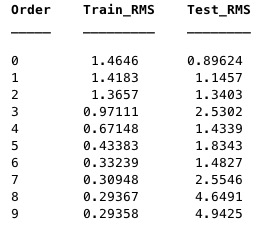
\includegraphics[width=0.8\linewidth]{2a1}
		\caption{}
		\label{fig:2a1}
	\end{figure}
	
	\paragraph{(b)}\mbox{}\\
	
	\begin{figure}[H]
		\centering
		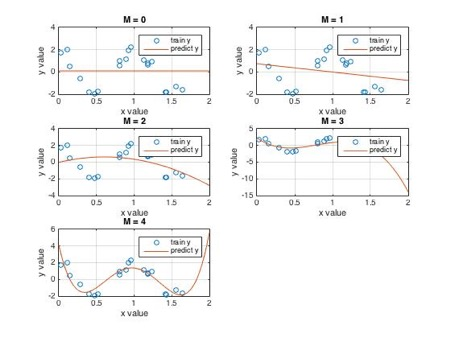
\includegraphics[width=0.8\linewidth]{2b1}
		\caption{}
		\label{fig:2b1}
	\end{figure}
	\begin{figure}[H]
		\centering
		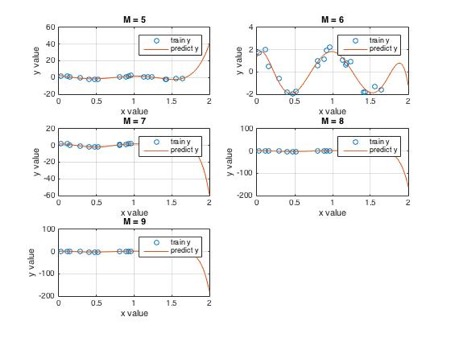
\includegraphics[width=0.8\linewidth]{2b2}
		\caption{}
		\label{fig:2b2}
	\end{figure}
	
	\paragraph{(c)}\mbox{}\\
	
	\begin{figure}[H]
		\centering
		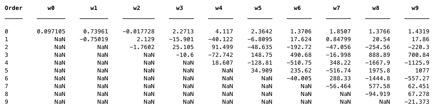
\includegraphics[width=1.2\linewidth]{2c1}
		\caption{}
		\label{fig:2c1}
	\end{figure}
	
	\paragraph{(d)}\mbox{}\\
	
	\begin{figure}[H]
		\centering
		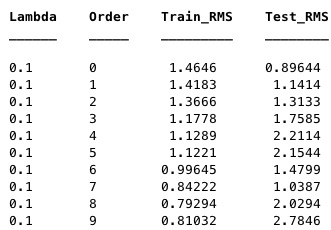
\includegraphics[width=0.8\linewidth]{2d1}
		\caption{}
		\label{fig:2d1}
	\end{figure}
	
	\paragraph{(e)}\mbox{}\\
	
	\begin{figure}[H]
		\centering
		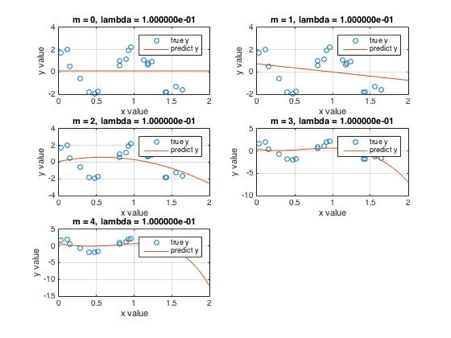
\includegraphics[width=0.8\linewidth]{2e1}
		\caption{}
		\label{fig:2e1}
	\end{figure}
	\begin{figure}[H]
		\centering
		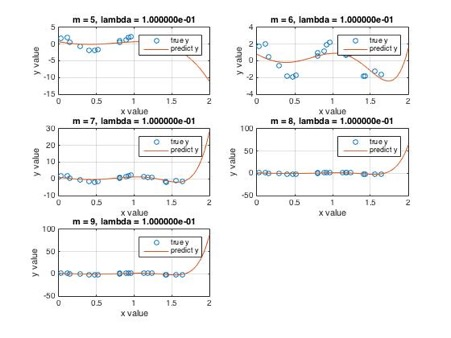
\includegraphics[width=0.8\linewidth]{2e2}
		\caption{}
		\label{fig:2e2}
	\end{figure}
	\begin{figure}[H]
		\centering
		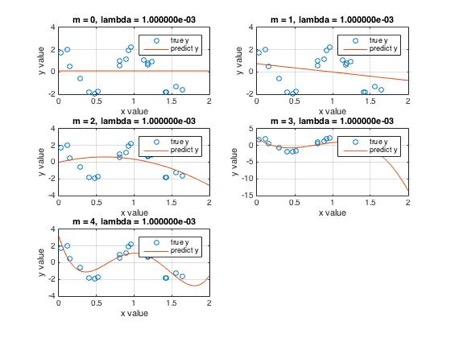
\includegraphics[width=0.8\linewidth]{2e3}
		\caption{}
		\label{fig:2e3}
	\end{figure}
	\begin{figure}[H]
		\centering
		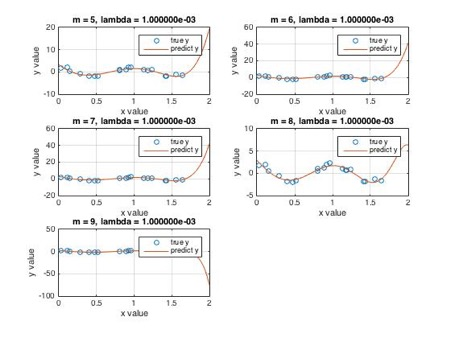
\includegraphics[width=0.8\linewidth]{2e4}
		\caption{}
		\label{fig:2e4}
	\end{figure}
	
	\paragraph{(f)}\mbox{}\\
	
	\begin{figure}[H]
		\centering
		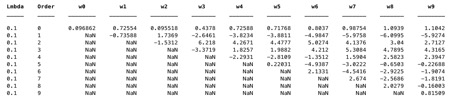
\includegraphics[width=1.2\linewidth]{2f1}
		\caption{}
		\label{fig:2f1}
	\end{figure}
	\begin{figure}[H]
		\centering
		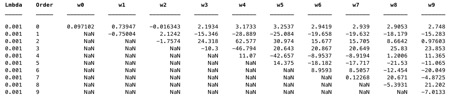
\includegraphics[width=1.2\linewidth]{2f2}
		\caption{}
		\label{fig:2f2}
	\end{figure}
	
	\paragraph{(g)}\mbox{}\\
	
	\subparagraph{a.}\mbox{}\\
	
	\begin{figure}[H]
		\centering
		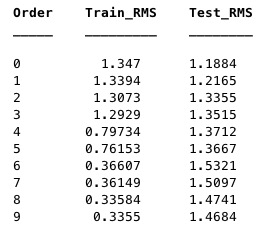
\includegraphics[width=0.8\linewidth]{2ga1}
		\caption{}
		\label{fig:2ga1}
	\end{figure}
	
	\subparagraph{b.}\mbox{}\\
	
	\begin{figure}[H]
		\centering
		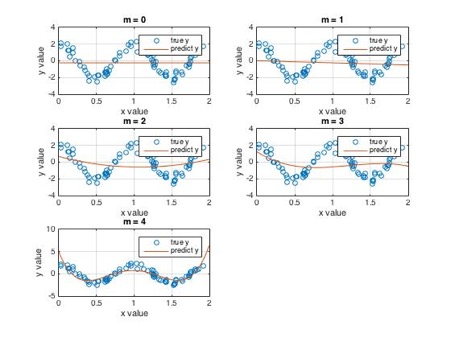
\includegraphics[width=0.8\linewidth]{2gb1}
		\caption{}
		\label{fig:2gb1}
	\end{figure}
	\begin{figure}[H]
		\centering
		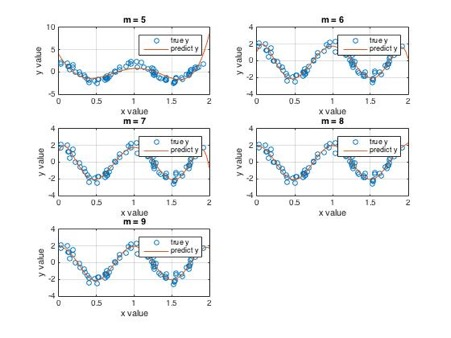
\includegraphics[width=0.8\linewidth]{2gb2}
		\caption{}
		\label{fig:2gb2}
	\end{figure}
	
	\subparagraph{c.}\mbox{}\\
	
	\begin{figure}[H]
		\centering
		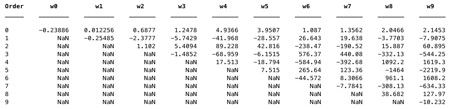
\includegraphics[width=1.2\linewidth]{2gc1}
		\caption{}
		\label{fig:2gc1}
	\end{figure}
	
	\subparagraph{d.}\mbox{}\\
	
	\begin{figure}[H]
		\centering
		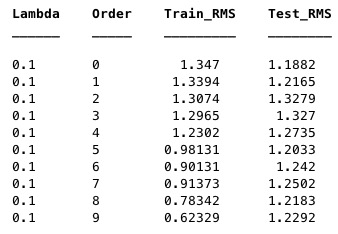
\includegraphics[width=0.8\linewidth]{2gd1}
		\caption{}
		\label{fig:2gd1}
	\end{figure}    
	\begin{figure}[H]
		\centering
		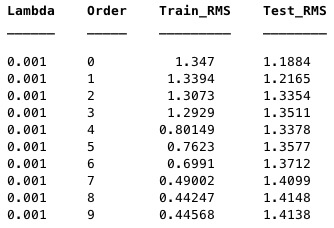
\includegraphics[width=0.8\linewidth]{2gd2}
		\caption{}
		\label{fig:2gd2}
	\end{figure}
	
	\subparagraph{e.}\mbox{}\\
	
	\begin{figure}[H]
		\centering
		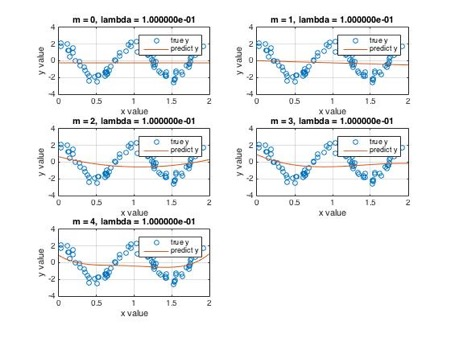
\includegraphics[width=0.8\linewidth]{2ge1}
		\caption{}
		\label{fig:2ge1}
	\end{figure}
	\begin{figure}[H]
		\centering
		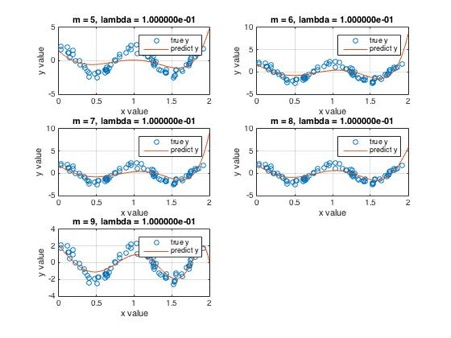
\includegraphics[width=0.8\linewidth]{2ge2}
		\caption{}
		\label{fig:2ge2}
	\end{figure}
	\begin{figure}[H]
		\centering
		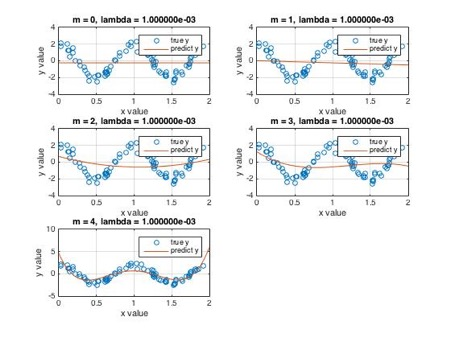
\includegraphics[width=0.8\linewidth]{2ge3}
		\caption{}
		\label{fig:2ge3}
	\end{figure}
	\begin{figure}[H]
		\centering
		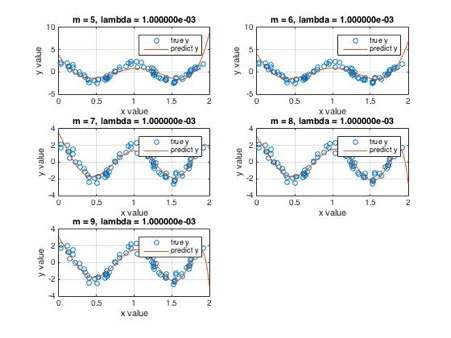
\includegraphics[width=0.8\linewidth]{2ge4}
		\caption{}
		\label{fig:2ge4}
	\end{figure}

	\subparagraph{f.}\mbox{}\\
	
	\begin{figure}[H]
		\centering
		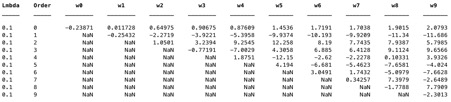
\includegraphics[width=1.2\linewidth]{2gf1}
		\caption{}
		\label{fig:2gf1}
	\end{figure}
	\begin{figure}[H]
		\centering
		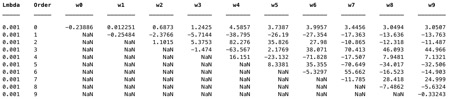
\includegraphics[width=1.2\linewidth]{2gf2}
		\caption{}
		\label{fig:2gf2}
	\end{figure}	
	
	\section{Application for Polynomial Regression}
	\paragraph{Overview}
	Like problem 2, using differential to get the parameter.

	\paragraph{(a)}\mbox{}\\
	
	\begin{figure}[H]
		\centering
		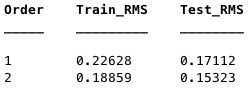
\includegraphics[width=0.8\linewidth]{3a1}
		\caption{}
		\label{fig:3a1}
	\end{figure}

	\paragraph{(b)}\mbox{}\\
	
	\begin{figure}[H]
		\centering
		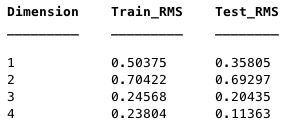
\includegraphics[width=0.8\linewidth]{3b1}
		\caption{}
		\label{fig:3b1}
	\end{figure}	
\end{document}
